%%
%% This is file `sigconf.tex',
%% generated with the docstrip utility.
%%
%% The original source files were:
%%
%% samples.dtx  (with options: `all,proceedings,sigconf')
%% 
%% IMPORTANT NOTICE:
%% 
%% For the copyright see the source file.
%% 
%% Any modified versions of this file must be renamed
%% with new filenames distinct from sigconf.tex.
%% 
%% For distribution of the original source see the terms
%% for copying and modification in the file samples.dtx.
%% 
%% This generated file may be distributed as long as the
%% original source files, as listed above, are part of the
%% same distribution. (The sources need not necessarily be
%% in the same archive or directory.)
%%
%%
%% Commands for TeXCount
%TC:macro \cite [option:text,text]
%TC:macro \citep [option:text,text]
%TC:macro \citet [option:text,text]
%TC:envir table 0 1
%TC:envir table* 0 1
%TC:envir tabular [ignore] word
%TC:envir displaymath 0 word
%TC:envir math 0 word
%TC:envir comment 0 0
%%
%% The first command in your LaTeX source must be the \documentclass
%% command.
%%
%% For submission and review of your manuscript please change the
%% command to \documentclass[manuscript, screen, review]{acmart}.
%%
%% When submitting camera ready or to TAPS, please change the command
%% to \documentclass[sigconf]{acmart} or whichever template is required
%% for your publication.
%%
%%
\documentclass[11pt,sigconf,nonacm]{acmart}
%%
%% \BibTeX command to typeset BibTeX logo in the docs
\AtBeginDocument{%
  \providecommand\BibTeX{{%
    Bib\TeX}}}

%% Rights management information.  This information is sent to you
%% when you complete the rights form.  These commands have SAMPLE
%% values in them; it is your responsibility as an author to replace
%% the commands and values with those provided to you when you
%% complete the rights form.

%% These commands are for a PROCEEDINGS abstract or paper.

%%
%%  Uncomment \acmBooktitle if the title of the proceedings is different
%%  from ``Proceedings of ...''!
%%
%%\acmBooktitle{Woodstock '18: ACM Symposium on Neural Gaze Detection,
%%  June 03--05, 2018, Woodstock, NY}


%%
%% Submission ID.
%% Use this when submitting an article to a sponsored event. You'll
%% receive a unique submission ID from the organizers
%% of the event, and this ID should be used as the parameter to this command.
%%\acmSubmissionID{123-A56-BU3}

%% (\include{caption} removed: there is no caption.tex and \include forces a page break)

%%
%% For managing citations, it is recommended to use bibliography
%% files in BibTeX format.
%%
%% You can then either use BibTeX with the ACM-Reference-Format style,
%% or BibLaTeX with the acmnumeric or acmauthoryear sytles, that include
%% support for advanced citation of software artefact from the
%% biblatex-software package, also separately available on CTAN.
%%
%% Look at the sample-*-biblatex.tex files for templates showcasing
%% the biblatex styles.
%%
%%
%% The majority of ACM publications use numbered citations and
%% references.  The command \citestyle{authoryear} switches to the
%% "author year" style.
%%
%% If you are preparing content for an event
%% sponsored by ACM SIGGRAPH, you must use the "author year" style of
%% citations and references.
%% Uncommenting
%% the next command will enable that style.
%%\citestyle{acmauthoryear}


%%
%% end of the preamble, start of the body of the document source.
\begin{document}

%%
%% The "title" command has an optional parameter,
%% allowing the author to define a "short title" to be used in page headers.
\title{The Performance Profiling of \texttt{pipe()}}

%%
%% The "author" command and its associated commands are used to define
%% the authors and their affiliations.
%% Of note is the shared affiliation of the first two authors, and the
%% "authornote" and "authornotemark" commands
%% used to denote shared contribution to the research.
\author{Arjun Anil, Aidan Liaw}
\email{aanil3@wisc.edu, aidan.liaw@student.uq.edu.au}

%%
%% By default, the full list of authors will be used in the page
%% headers. Often, this list is too long, and will overlap
%% other information printed in the page headers. This command allows
%% the author to define a more concise list
%% of authors' names for this purpose.
\renewcommand{\shortauthors}{Anil et al.}

%%
%% The abstract is a short summary of the work to be presented in the
%% article.
% \begin{abstract}
%   The POSIX anonymous \texttt{pipe()} (referred to as pipe henceforth) inter-process communication (IPC) method is a common way to send data between parent and child. This is because of its simple setup semantics (when using \texttt{fork}), built-in synchronisation, and automatic resource management. It performance however, is often overlooked. In doing so we explore the rabbit hole of performance profiling in Linux via the \texttt{perf}, \texttt{strace}, and \texttt{ftrace} functions, and ultimately conclude that [WRITE CONCLUSION.]
% \end{abstract}

%%
%% The code below is generated by the tool at http://dl.acm.org/ccs.cfm.
%% Please copy and paste the code instead of the example below.
%%

%%
%% Keywords. The author(s) should pick words that accurately describe
%% the work being presented. Separate the keywords with commas.

%%
%% This command processes the author and affiliation and title
%% information and builds the first part of the formatted document.
\maketitle


\section{Introduction}

The POSIX standard defines \texttt{pipe()} as a function that creates an anonymous pipe and places two file descriptors, for the read and write ends, in its argument \cite{posix2024}. Through the Virtual File System a pipe is used with \texttt{read()} and \texttt{write()} \cite{LinuxVfsDocs,slideshare_linux_pipes}, and its kernel buffers are guarded by a mutex. Two sizes matter: \texttt{PIPE\_BUF}, up to which a write is atomic, i.e.\ never interleaved with another writer's data \cite{linux_man_pipe7}, and the finite pipe capacity, past which a blocking producer sleeps until a consumer drains the pipe. This paper analyses \texttt{pipe()}: we measure its latency and throughput and use \texttt{perf}, \texttt{strace} and \texttt{ftrace} to explain where the time goes.

\section{Experiment}

\subsection{Variables}

\begin{itemize}
    \item The message size, as suggested by the instructor: 4B, 16B, 64B, 256B, 1024B, 4096B, 16384B, 65536B, 262144B and 524288B. 4096B matches \texttt{PIPE\_BUF}, which is preset \cite{linux_limits_h}, and 65536B the pipe capacity \texttt{PIPE\_LENGTH}, which we leave at the kernel default.
    \item The number of measurements: 20 warmup and 2000 timed round trips per size in each of 5 runs (latency); 3 transfers of 64\,MiB per size in each of 5 runs (throughput; 4B and 16B are capped at 2,000,000 chunks).
    \item Both processes run under \texttt{SCHED\_FIFO} at priority 99, the parent on CPU0, the child on CPU1 and the profiler on CPU2, with the frequency pinned to 4 GHz.
    \item Blocking I/O: no \texttt{O\_NONBLOCK}, so tasks sleep instead of spinning.
\end{itemize}

\subsection{Hypotheses}

\begin{enumerate}
    \renewcommand{\labelenumi}{\arabic{enumi}.}
    \item The variance in data measurements between runs should be minimal, given the care taken to ensure process isolation.
    \item Performance will get worse for data sizes above \texttt{PIPE\_BUF}, which we expected might split a write into several operations, and for data sizes above \texttt{PIPE\_LENGTH}, as the producer must stall until the consumer drains the pipe.
\end{enumerate}

\subsection{Apparatus}

The laptop has an Intel Core Ultra 7 258V and runs Fedora Linux 44, kernel 7.1.8; only its four P-cores are used.

\paragraph{Timer.} Timer resolution is the smallest non-zero difference between back-to-back reads. \texttt{gettimeofday()} resolves 1\,$\mu$s and \texttt{CLOCK\_\allowbreak MONOTONIC\_\allowbreak COARSE} 1\,ms, too coarse for a message of about a microsecond, while \texttt{CLOCK\_MONOTONIC} (11\,ns) and \texttt{rdtsc} (7.3\,ns) are not. We use \texttt{rdtsc}, whose counter is invariant on this CPU and read in the parent only, so each latency is a difference of two reads on one core; cycles are converted to time by calibrating against \texttt{CLOCK\_MONOTONIC} (3.302\,GHz). Around a \texttt{sleep(2)} the three fine timers agree to within 10.5\,$\mu$s, and \texttt{gettimeofday()}, the less accurate reference, is within 1.9\,$\mu$s of \texttt{CLOCK\_MONOTONIC}.

\paragraph{Procedure.} For latency, a parent and a child (\texttt{fork()}) are connected by two pipes and the child echoes each message; the one-way latency is half the round trip, as the counters of two cores cannot be compared. For throughput the parent streams chunks and the child returns one acknowledgement byte after the whole transfer. Noise can only add time, so we report the minimum latency and the best throughput \cite{smith1988,heiser_benchmarking_crimes}. The profilers slow the benchmark, so they run separately and only counts and proportions are used: \texttt{perf} \cite{perf_wiki,redhat_perf_raw_events}, \texttt{strace} \cite{linux_man_strace} and \texttt{ftrace}, which also sees the kernel calls \texttt{strace} cannot \cite{linux_ftrace_docs,so:ftrace_vs_strace}.

\section{Results}

\begin{figure}[t]
    \centering
    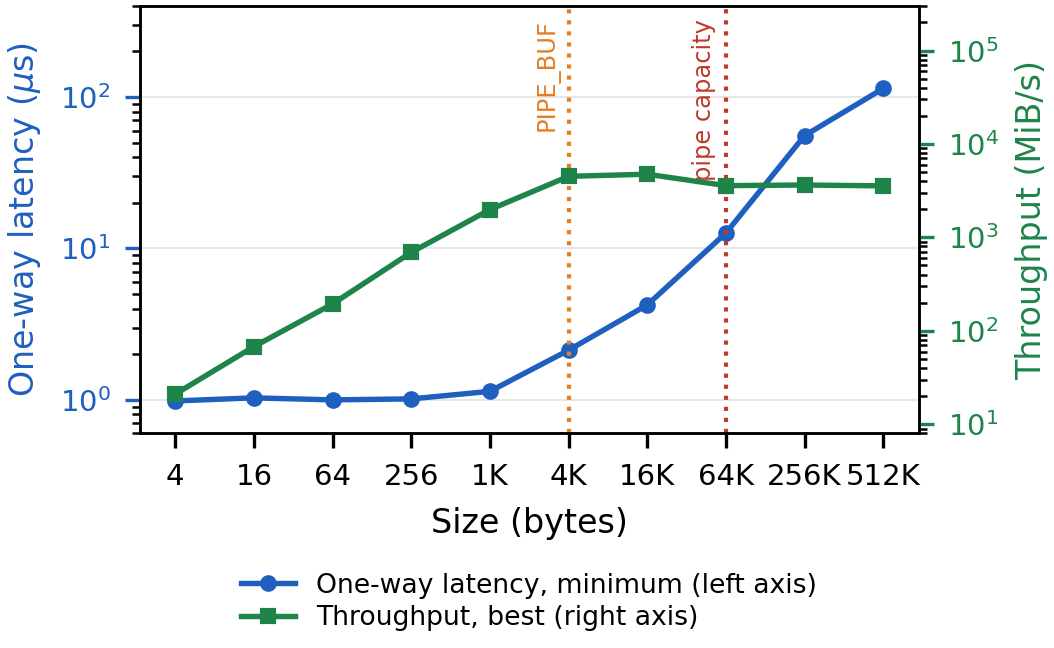
\includegraphics[width=\columnwidth]{latency_throughput.png}
    \caption{Minimum one-way latency (left axis) and best throughput (right axis) versus transfer size; dotted lines mark \texttt{PIPE\_BUF} and the pipe capacity.}
    \label{fig:lat-tp}
    \Description{Latency and throughput against message size on two logarithmic axes.}
\end{figure}

\begin{figure}[t]
    \centering
    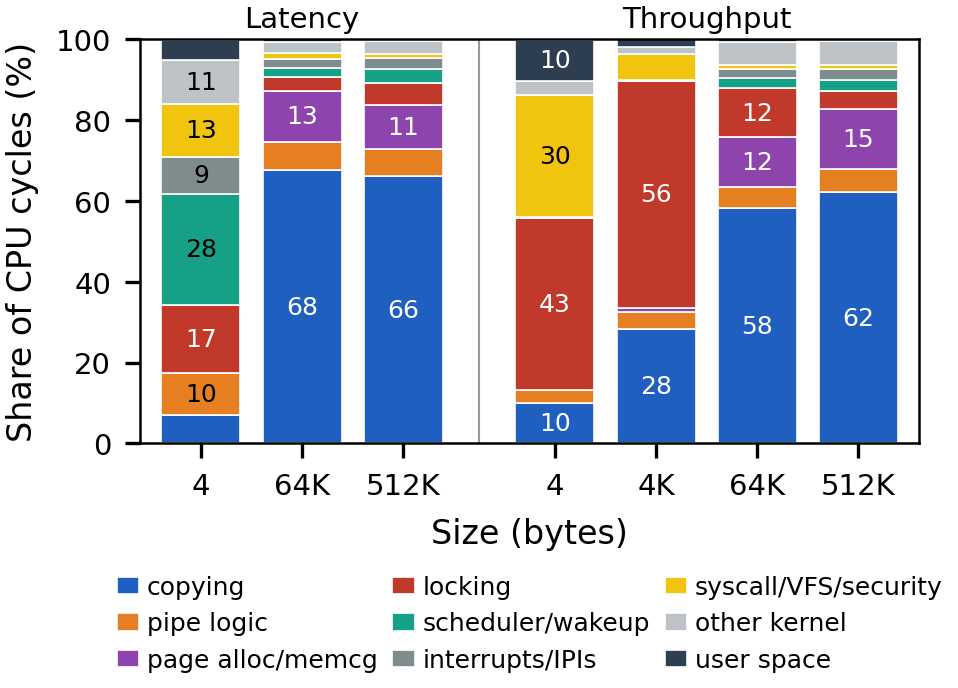
\includegraphics[width=\columnwidth]{fig_breakdown.png}
    \caption{Share of the CPU cycles per component, for latency and throughput.}
    \label{fig:breakdown}
    \Description{Stacked bars of the CPU cycle shares per component for latency and throughput.}
\end{figure}

\begin{figure}[t]
    \centering
    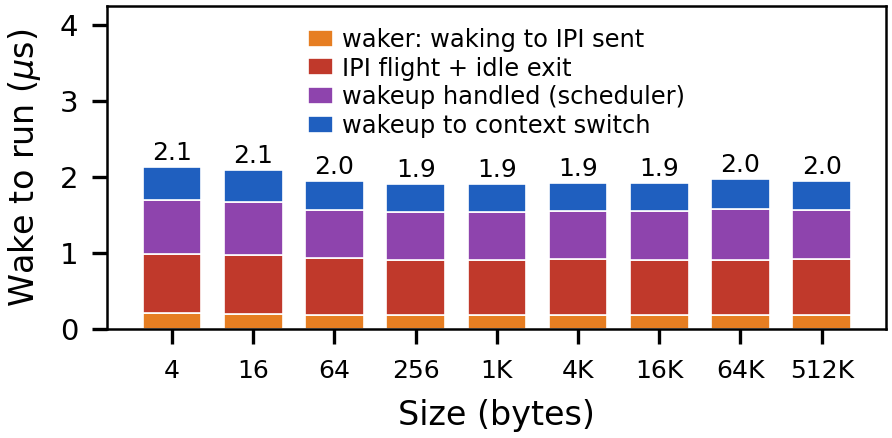
\includegraphics[width=\columnwidth]{fig_wakeup.png}
    \caption{Phases of a wakeup (median, latency experiment, traced; 256KB omitted, as only 43\% of its wakeups found the core idle).}
    \label{fig:wakeup}
    \Description{Stacked bars of the four wakeup phases per message size.}
\end{figure}

Figure~\ref{fig:lat-tp} shows that a small message takes about 1\,$\mu$s one way (0.98\,$\mu$s at 4B), stepping up to 2.12\,$\mu$s at 4KB, and beyond the pipe capacity latency is roughly proportional to the size (113.9\,$\mu$s at 512KB). Throughput rises from 21\,MiB/s (4B) to a peak of 4,742\,MiB/s at 16KB, is 25\% lower at 64KB (3,578\,MiB/s) and stays there up to 512KB. The minima reproduced to within 0.9--9.7\% (latency) and 5.8--14\% (throughput, chunks of 1KB and larger; 29--39\% for 4B and 16B) across five runs.

\section{Where the Time Goes}


\texttt{strace} shows one \texttt{write()} per message at every size. A round trip of up to 64KB causes 2 context switches, 2 wakeups and 2 inter-processor interrupts; 256KB and 512KB cause 14 and 30 context switches, i.e.\ $2(2n-1)$ for $n$ pipe capacities, because the writer fills the pipe and sleeps until the reader drains it. For 4B the median round trip is 3.06\,$\mu$s, but the tasks run for only 2.11\,$\mu$s: for 0.95\,$\mu$s (31\%) neither runs, as a sleeping core is woken.

In Figure~\ref{fig:breakdown}, for 4B no component dominates: scheduling and wakeup take 27.5\%, locking 16.8\% and copying only 7.1\%. At 64KB and 512KB copying takes 68\% and 66\%. Waking to running takes 1.9--2.1\,$\mu$s at every size (Figure~\ref{fig:wakeup}): a fixed cost paid twice per round trip. The \texttt{ftrace} call tree agrees: at 4B reads are dominated by the blocked \texttt{schedule}, writes by the wakeup chain.

Streaming works as a pipeline: for chunks of 64B to 16KB there are almost no context switches and 1.9--2.0 cores are busy (CPU time over wall time). From 64KB each chunk causes 2 to 16 context switches and only 0.86--0.91 cores are busy, as the writer fills the pipe and sleeps. The cost per KiB even falls (1,741 to 991 cycles), but with half the parallelism throughput drops. At 4KB the tasks spin on the pipe mutex (56\% locking).

\section{Discussion and Conclusion}

The first hypothesis holds only in part: the minima reproduced within 10--14\%, but the median small-message round trip is 56\% above the minimum. Of the second, the \texttt{PIPE\_BUF} half is not supported: every message is a single \texttt{write()} and throughput peaks at 16KB instead of falling at 4KB. Latency does step up at 4KB (the median round trip grows by 2.1\,$\mu$s from 1KB, half of it with neither task running), which we cannot explain. The capacity half is supported: past 64KB the writer must sleep and throughput falls by 25\%.

Small messages are therefore a scheduling problem and large messages a copying problem. These results come from a single laptop with the frequency pinned at 4\,GHz. Two further caveats are that \texttt{SCHED\_FIFO} and tracing add overhead of their own, and that we did not vary the pipe capacity or page size.

\clearpage
\bibliographystyle{ACM-Reference-Format}
\bibliography{sample-base}

\end{document}
\endinput
